\documentclass[10pt]{article}


%\usepackage{fullpage}
\usepackage{amsmath}
\usepackage{graphicx}
\usepackage{extpfeil}

   \usepackage{cite}

%\usepackage{draftcopy}

%\usepackage{multirow}

\newcommand{\xx}{\mathbf{x}}



\usepackage[outercaption]{sidecap}    



\title{Statistical testing for GBM}

%%%%%%%%%%%%%%%%%%%%%%%%%%%%%%%%%%%%%%%%%
\begin{document}

    % first the title is needed


\date{\today}
\author{G. Caravagna and G. Sanguinetti and A. Sottoriva}

\maketitle



We have a tumour with  multi-region sequencing of samples {\sf T1},  {\sf T2}, $\ldots$ ({\em tumour})  and of    {\sf M} ({\em margin}). For each sample we have available:
\begin{itemize}
\item WES at average 100x;
\item TES1 and TES2, two targeted deep-sequencing panels at 3000x, built as explained above.
\end{itemize}

We observe a phylogenetic reconstruction in which  {\sf M} is ancestral to 
 {\sf T1},  {\sf T2}, $\ldots$, and want to compute the evidence for that, given our sequencing data, via a suitable statistical test. 

 \paragraph{Test construction.}
If {\sf M} is ancestral to  {\sf T1},  {\sf T2}, $\ldots$ we expect to see one (or more) clonal mutations in {\sf T1},  {\sf T2}, $\ldots$, that are missing in  {\sf M}. The test  consists in providing evidence for a negative call of such mutations in the margin, given the expected frequency that a clonal mutation   should have
 (i.e., quantifying the probability that a non-observed mutation is a {\em true negative}).  The test will get strength (i.e., significance in rejecting $H_0$) proportionally to the coverage for clonal mutations, and the purity of the sample.

We  discuss the p-value for the test of a single mutation, and then a correction for multiple hypotheses testing.
Consider $x$ a   clonal\footnote{We consider  $x$   clonal when it has variant allele frequency above    $0.20$ in all the samples {\sf T1},  {\sf T2}, $\ldots$, after that we have corrected the   frequency estimates for purity of the WES sample. If the variant is also present in one of the two panels, we prioritize clonality assessment from those panel.
} 
mutation  in   {\sf T1},  {\sf T2}, $\ldots$  To be considered for downstream analysis, we require $x$ to be 
 ``missing'' in the margin (i.e., it must have 0 mutated reads in {\sf M}) and a minimum coverage of 100 in the target panels,  we shall use the TES1 and TES2 targeted panels to estimate if a clonal $x$ is tested. Then any such $x$ would have expected variant allele frequency 
\begin{align}
v_x = \dfrac{r_x}{c_x}  && 
\text{where }\;
 r_x \sim {\sf BetaBinomial}(c_x\mid \mu, \rho)
\end{align}
where:
\begin{itemize}
\item $c_x$ is the coverage at $x$, and $r_x$  the number of reads with the mutant allele;
\item $(\mu, \rho)$ are the MLE of a Beta-Binomial random variable describing overdispersed read counts for clonal mutations.
\end{itemize}
We  fit  Beta-Binomial counts from each one of our WES samples of  {\sf T1},  {\sf T2}, $\ldots$, and test them {\em independently} (however, correcting for multiple tests at the end of the procedure). 

Since we have a statistical model for the expected number of mutated reads for a clonal mutation, the p-value of our test (i.e., the null model) is just the probability of seeing 0 mutant reads for $x$ in {\sf M}, where $x$ suppose it has coverage $m_x$.
%
%
%, which has lower coverage -- and thus possibly understimates the frequency of clonal mutations, resulting in more overdispersed values especially if the sample has low purity. Thus, since we have $0$ mutated reads in {\sf M},
%
The hypothesis $H_0$ has p-value
\[
H_0: p = {\sf BetaBinomial}(0 \mid m_x \cdot \pi ; \mu, \rho) 
\]
%where:
% 
%\[
%\hat{m}_x = m_x \cdot \pi 
%\]
%
which is the probability of observing 0 reads at coverage $m_x$ -- in {\sf M} from one of the two targeted panels --  adjusted for sample purity  $\pi$, given $(\mu, \rho)$  the parameters fit  for clonal mutations. This probability gives  a simple curve as a function of the coverage value, which represents the power of the test.

Observe that correction for purity is done by shifting the coverage estimates. In practice, we throw away $(1-\pi)$ percent of the reads mapping to $x$ in the margin. This is correct, since given that $x$ has $0$ mutant reads in the margin, we are not biasing any estimate for $x$ (its VAF still remains $0$). Clearly, the lower the purity the higher has to be coverage of $x$ to pass the test.

Correction for multiple hypotheses testing is straightforward with a Bonferroni FWER model (which is also the stringent possible correction); when we  test for $w$ mutations in $r$ regions, we accept only mutations that have p-value below $p_\ast/(wr)$ for all the possible  settings of training and test. As usual, we set   $p_\ast = 0.05$ as our baseline confidence. 

%
%
%
%
%
%
%\begin{figure}[t]\centerline{
%\includegraphics[width=18cm]{gapstat}}
%\caption{{\bf Example data.} left: $n=340$ points generated from a mixture of 3 univariate Gaussian mixtures, plot in order of generation (x-axis). The mixtures have $\mu= 0, 10, 4$, and $\sigma^2=1, 10, 40$, rendering hard distinguishing the $k=3$ clusters. right: value of the gap statistics for $k=1,\ldots, 15$ and $B=10$. With these values {\sf globalmax}, {\sf Tibs2001SEmax} and {\sf firstSEmax} indentify $k_\ast = 2$; for instance  {\sf Tibs2001SEmax} computes $k_\ast=2$ since  $G_n(2) \geq G_n(3) - s_{3}$ but $G_n(1) < G_n(2) - s_{2}$.
%}
%\label{fig:example}
%\end{figure}
%
%
%\begin{figure}[t]\center
%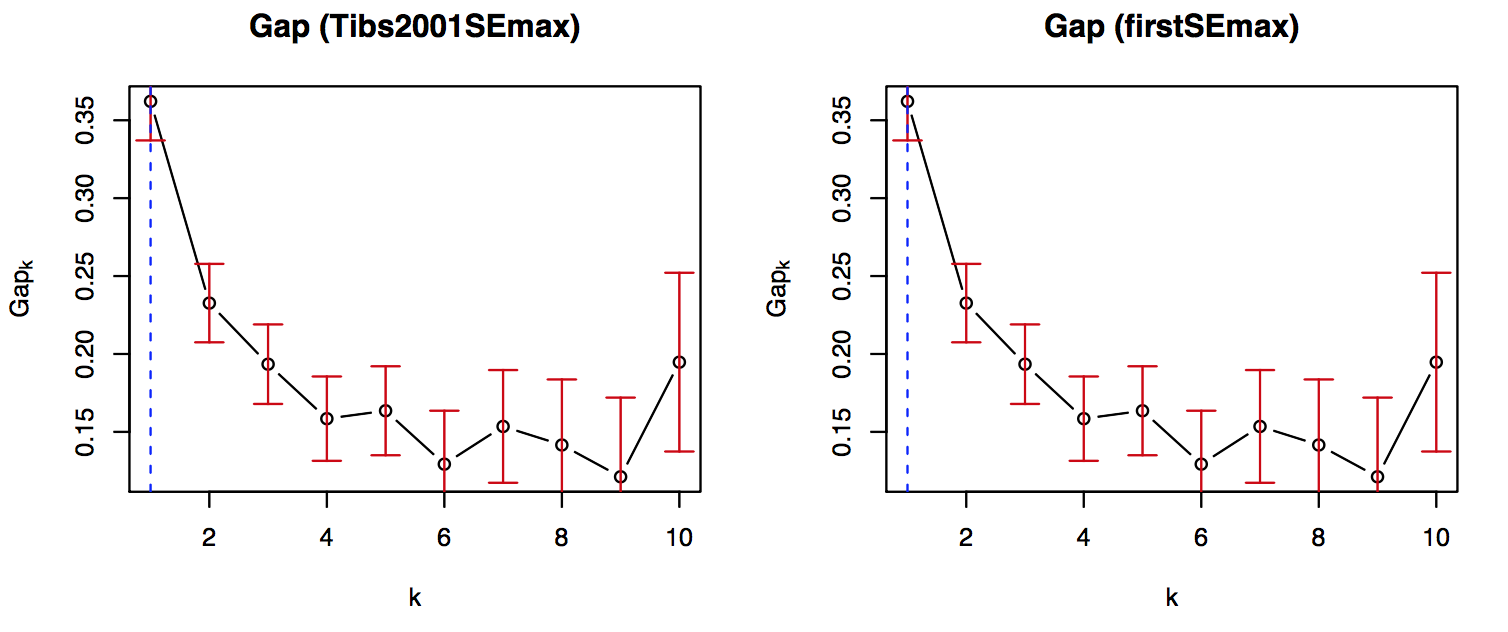
\includegraphics[height=5cm]{gap3}
%\caption{{\bf PD3851 data} left: if we use the gap-statistics maximization criterion, we have $k_\ast = 6$. right: by the one standard error rule, we would have $k_\ast = 3$ since $G_n(3) \geq G_n(4) - s_{4}$ but $G_n(2) < G_n(3) - s_{3}$.
%}
%\end{figure}



\end{document}
